\documentclass[11pt,twoside]{report}
\usepackage{preamble}
\graphicspath{{../img/ch5/}}
\setcounter{chapter}{5}

\begin{document}

\chapter{Modelling the Zebrafish}
\label{chapter:fish_model}


\epigraph{子非魚\; 安知魚之樂\\[1ex]You are not a fish, how could you know about the happiness of the fish}{莊子}

This chapter will introduce some computer simulation work for reproducing the observed experimental results. Computer simulation, altogether with theoretical calculation, experimental observation and democratic voting\marginfootnote{Jokingly, the existence of liquid--solid phase transition were put on a vote by George Uhlenbeck on a meeting in 1957 \cite{battimelli2018}.}, manifested itself as a powerful tool to answer questions about the nature of complex systems.

\section{Introduction}

In this section, different agent-based\marginfootnote{The moving individuals in the model can take different names, like the ``particles'', ``animals'', and ``agents''. The term ``agents'' will be used in this chapter for consistency.} models will be discussed in order to mimic the observed behaviours of zebrafish. A simple model would capture the essence of the fish system, while a detailed model could re-create the behaviours of fish in very realistic way. A good and accurate model would give people extra insights about the fish, enabling the creation of theories to predict the behaviours of the systems under different conditions, just like one can predict the volume of ideal gas under different temperatures, knowing the corresponding equation of states.

Thanks to the development of the computer hardwares and the softwares, one can write a programming that simulate different type of models very easily. The simulation method for different models and details would be introduced in this chapter, and I will compare the simulation result with the experimental observations.

But what is the interesting property that we want to simulate? The full phase--space of $N$ fish has the dimension of $6 \times N$, and the amount of features, to be calculated from the $6 \times N$ numbers, can be considerable. In my own opinion, there is no correct answer. But we can take our trust in \emph{democracy}, and follow the popular options.

Thinking about the animals exhibiting collective behaviour, the popular idea (in 2020s) is to study their \emph{ordering process}. Namely, we study how the animals align their velocities to form synchronised (or disorderd) movements. As the animals order their moving directions, other ordering processes are also happening, for instance the unification of opinions. Hence, I will be modelling the animal behaviours focusing on their ordering process.


\section{Simulation Methods}

\subsection{Monte--Carlo Simulation}

\begin{tcolorbox}[
title=Monte--Carlo Sweep,
enlarge bottom by=0.5em,
enlarge top by=0.5em,
]
\label{alg:graph-vnm}
\begin{algorithmic}
\Procedure{mc-sweep}{}
\For {$i \in \{0 \dots n\}$}
\State change state of agent $i$
\EndFor
\EndProcedure
\end{algorithmic}
\end{tcolorbox}


\begin{tcolorbox}[
title=General Description of MC simulation,
enlarge bottom by=0.5em,
enlarge top by=0.5em,
]
\label{alg:graph-vnm}
\begin{algorithmic}
\Procedure{mc-sim}{}
\State System $\gets$ initial state
\Repeat
	\State Monte-Carlo Sweep
\Until {System is stable} \\

\State Result $\gets$ \{ \}
\Repeat
	\State Monte-Carlo Sweep
	\State Calculate Q, and put Q in Result
\Until {Statistic is good enough}
\State \textbf{return} Result
\EndProcedure
\end{algorithmic}
\end{tcolorbox}


\subsection{Brownian Dynamic Simulation}


\begin{tcolorbox}[
title=General Description of BD simulation,
enlarge bottom by=0.5em,
enlarge top by=0.5em,
]
\label{alg:graph-vnm}
\begin{algorithmic}
\Procedure{bd-sim}{}
\State System $\gets$ initial state
\Repeat
	\State advance $\delta t$
\Until {System is stable} \\

\State Result $\gets$ \{ \}
\Repeat
	\State advance $\delta t$
	\State Calculate Q, and put Q in Result
\Until {Statistic is good enough}
\State \textbf{return} Result
\EndProcedure
\end{algorithmic}
\end{tcolorbox}

Notice the structure of BD simulation and MC simulation is the same. The only difference comes from the way to change the state of the system. Hence, for abstracted model like the voter model I applied the MC procedure while for realistic model I would apply the BD procedure.

\subsection{Molecular Dynamic and other Methods}

It is worth mentioning other simulation methods. A technique similar to the BD simulation is the molecular dynamic simulation. % (Some words about LAMMPS)
Another elegant method is the event--driven molecular dynamic simulation, which is widely used to simulate the idealised hard sphere system, where the agents have different diameters and they can not overlap with each other. The key part of the event--driven MD simulation is to determine the configuration when different collision events happen. This method is also used to simulate active matter system with different interactions at different length scales, for instance in.

\section{Ordering on a Graph: Voters and Vectorial Networks}

% introduce the very limited graph theory (that I happen to know!) here.

The very interesting ordering phenomena in the nature are often treated as the results of interactions between different agents. For instance, the coordinated movement of birds can rise from the velocity alignment between birds that are close to each other. More abstractly, the human decision are also affected by friends, and such interaction leads to collective decision making.

\subsection{Introduction to the Graph}

The popular tool to summarise the interaction of different agents is the \emph{graph}. The graph is.

Here we will focus on a typical type of graph in which each node will have a fixed number, $K$, of edges. This property is termed as ``each node is of degree $K$'' in the graph theory.\marginfootnote{
The graph in which every node has a degree $k$ is called \emph{$k$--regular} graph. However, in a common context the regular graph is implecitly \emph{simple}. A simple graph is a undirected graph with no self--loop nor multiple links between two nodes.
} Figure \ref{fig:graph-vnm} shows some example of these graphs, altogether with their matrix representations. The graphs are directional, and the edge from node $i$ to node $j$ specifies the alignment interaction, in which agent $i$ will align with agent $j$ (but not the other way around).

In order to mimic the evolution of the relation between agents, the graph is drawn uniformly from all valid possibilities during the simulation. That is to say, agent $i$ will have different neighbours during the simulation. There is a simple rejection--free method to generate such graph, and this method is presented in the following algorithm.

\begin{tcolorbox}[
title=Algorithm to generate the graph for VNM,
enlarge bottom by=0.5em,
enlarge top by=0.5em,
]

\label{alg:graph-vnm}
\begin{algorithmic}

\Procedure{rand-graph-vnm}{k, n}
\State Nodes $\gets \{0 \dots n-1 \}$
\State Edges $\gets \{\}$
\For {$i_1 \gets 1, n$}
	\State Selection $\gets$ \{\}
	\Repeat
		\State $i_2 \gets$  randomly choose from Nodes
		\If {$i_2$ not in Selection}
			\State put $i_2$ in Selection
			\State put $(i_1, i_2)$ in Edges
		\EndIf
	\Until size(Selection) = k
\EndFor
\State \textbf{return} (Nodes, Edges)
\EndProcedure
\end{algorithmic}

\end{tcolorbox}


\begin{SCfigure}
  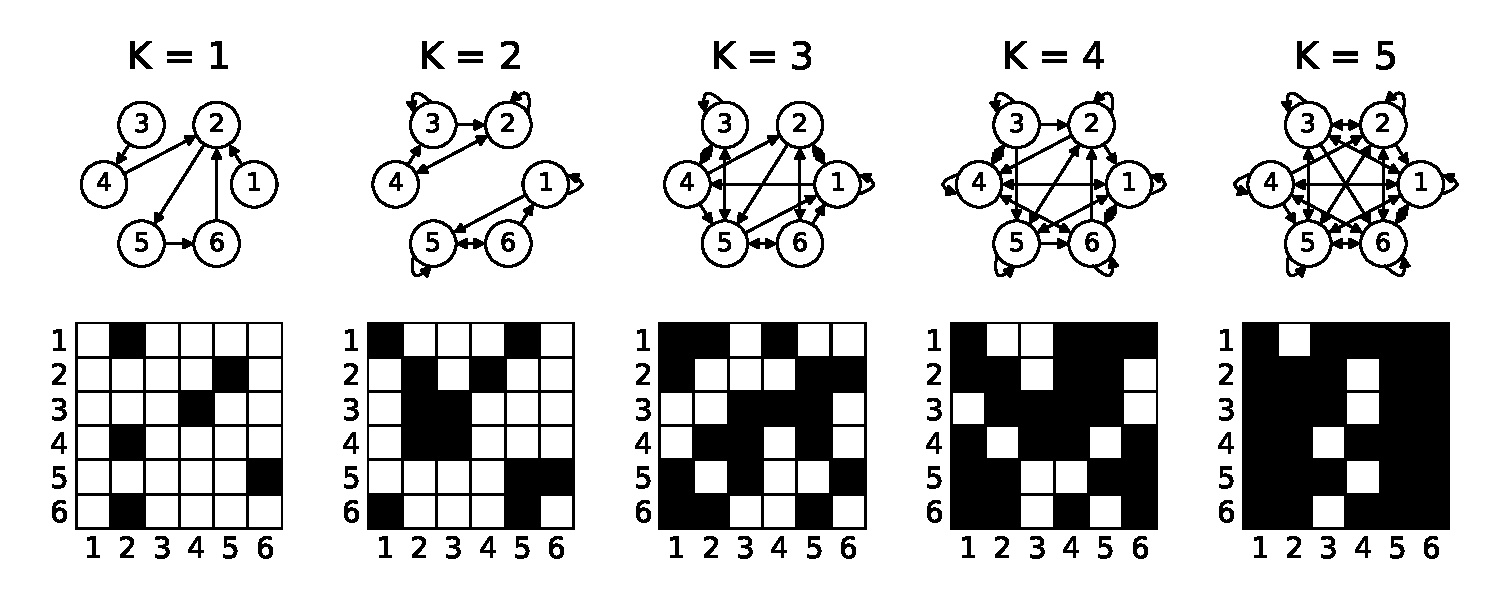
\includegraphics[width=\linewidth]{graph-vnm}
  \caption{Graph and matrix representation of the vectorial network model, with increasing connection number ($K$). The top row illustrate the relationship between 5 agents. And the arrow from $i$ to $j$ indicates that agent $i$ will align with agent $j$. The bottom row indicates the adjacency matrices of these graphs. }
  \label{fig:graph-vnm}
\end{SCfigure}

Notably, the topology of the graph can be changed. For instance, we can force each node to interact with itselves. As well as forcing the graph to be un--directed, where the edge $i \rightarrow j$ and edge $i \leftarrow j$ must present at the same time. Figure \ref{fig:graph-regular} presented some examples of this type of graph.

\begin{SCfigure}
  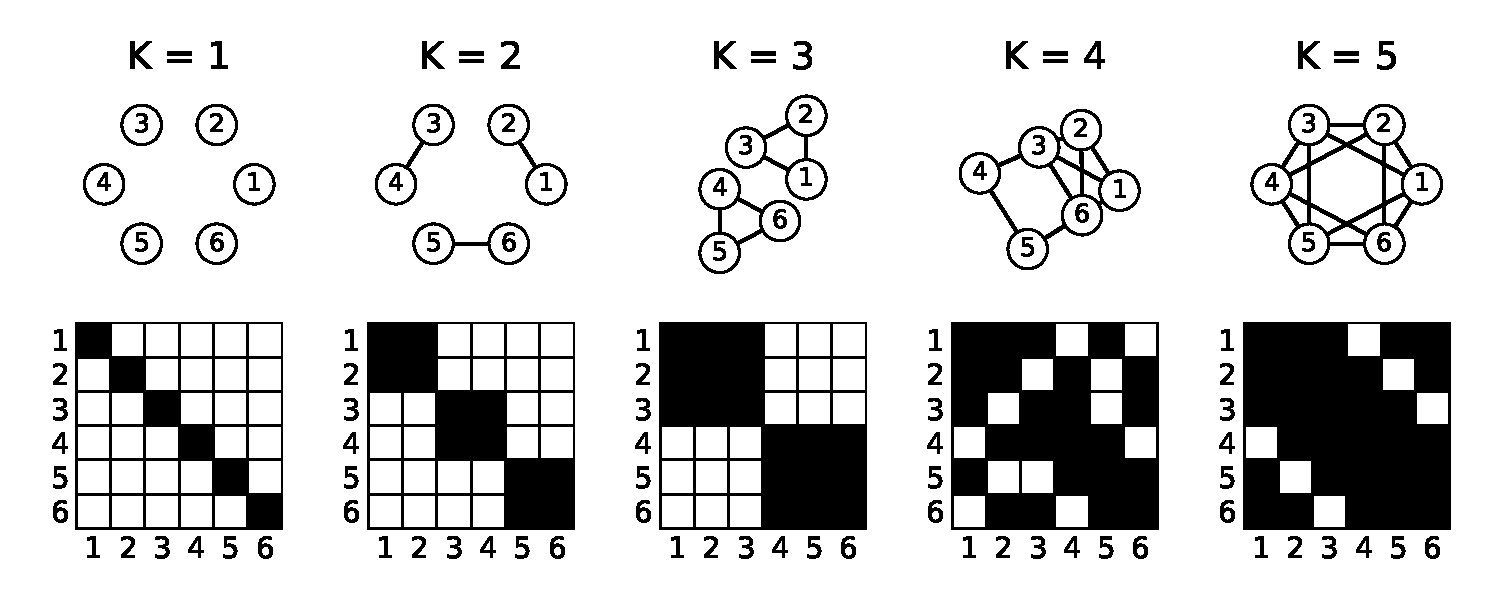
\includegraphics[width=\linewidth]{graph-regular}
  \caption{Graph and matrix representation of the vectorial network model with extra topological constrains. The sub--figures have increasing connection number ($K$) from left to right. The top row illustrate the relationship between 5 agents. And the arrow from $i$ to $j$ indicates that agent $i$ will align with agent $j$. The bottom row indicates the adjacency matrices of these graphs. }
  \label{fig:graph-regular}
\end{SCfigure}

Generating random graphs that meets the constrains of cgVNM is not easy. But we can at least resort to the rejection algorithm (Algorithm \ref{alg:graph-cgvnm}).

\begin{tcolorbox}[
title=Rejection Algorithm to generate graphs with constrains,
enlarge bottom by=0.5em,
enlarge top by=0.5em,
]

\label{alg:graph-cgvnm}
\begin{algorithmic}

\Procedure{rand-graph-cgvnm}{k, n}
\State succeed $\gets$ false
\Repeat
	\State (Nodes, Edges) $\gets$ rand-graph-vnm(k, n)
	\State succeed $\gets$ Edges satisfy all constrains
\Until succeed
\State \textbf{return} (Nodes, Edges)
\EndProcedure
\end{algorithmic}
\end{tcolorbox}

\noindent However, the rejection method can be extremely slow when the rejection ratio is high. In practice, the rejection method is not practical for large scale simulation. In my actually simulation, a faster algorithm was used \cite{kim2003book}. The behaviour of the cgVNM is very similar to the VNM.

\subsection{The Majority Voter Model}

The majority voter model\marginfootnote{The majority voter model is introduced also because it is reminiscent of the celebrated Ising model. However this thesis will not refer to the Ising model, in order to comfort the unfamiliar readers. However I would like to point out the similarity between the two order parameters: the \emph{polarisation} of the active matter models and the \emph{magnetisation} of the Ising model.}
 treats each agent as a binary variable (noted as $v_i$) that takes the value of $+1$ and $-1$. And each agent will interact with its neighbours with the following interaction rule \cite{pimentel2008PRE}. 
 
$$
v_i(t+1) = \left\{ \begin{array}{ll}
\mathrm{sgn} \left[ U_i(t) \right]
& (\textrm{probability} = 1-\eta/2) \\[1em]
-\mathrm{sgn} \left[ U_i(t) \right]
& (\textrm{probability} = \eta/2)
\end{array}
\right.
$$

\noindent where the $\textrm{sgn}[ \cdot ]$ is the operator that takes the sign of the expression inside the squared brackets. The symbol $\eta$ represent the noise, and taking the value between 0 and 1. The term $U_i(t)$ represent the majority voting result of the neighbours of agent $i$. The expression of $U_i(t)$ is written as,

$$
U_i(t) = \frac{1}{K} \sum_{j \in S_i} v_j(t).
$$

\noindent And the symbol $S_i$ corresponds to the neighbours of agent $i$, and it is determined by the underlying graph of the model.
 
The behaviour of the voter model is presented in Fig.\ \ref{fig:voter}.

\begin{SCfigure}
  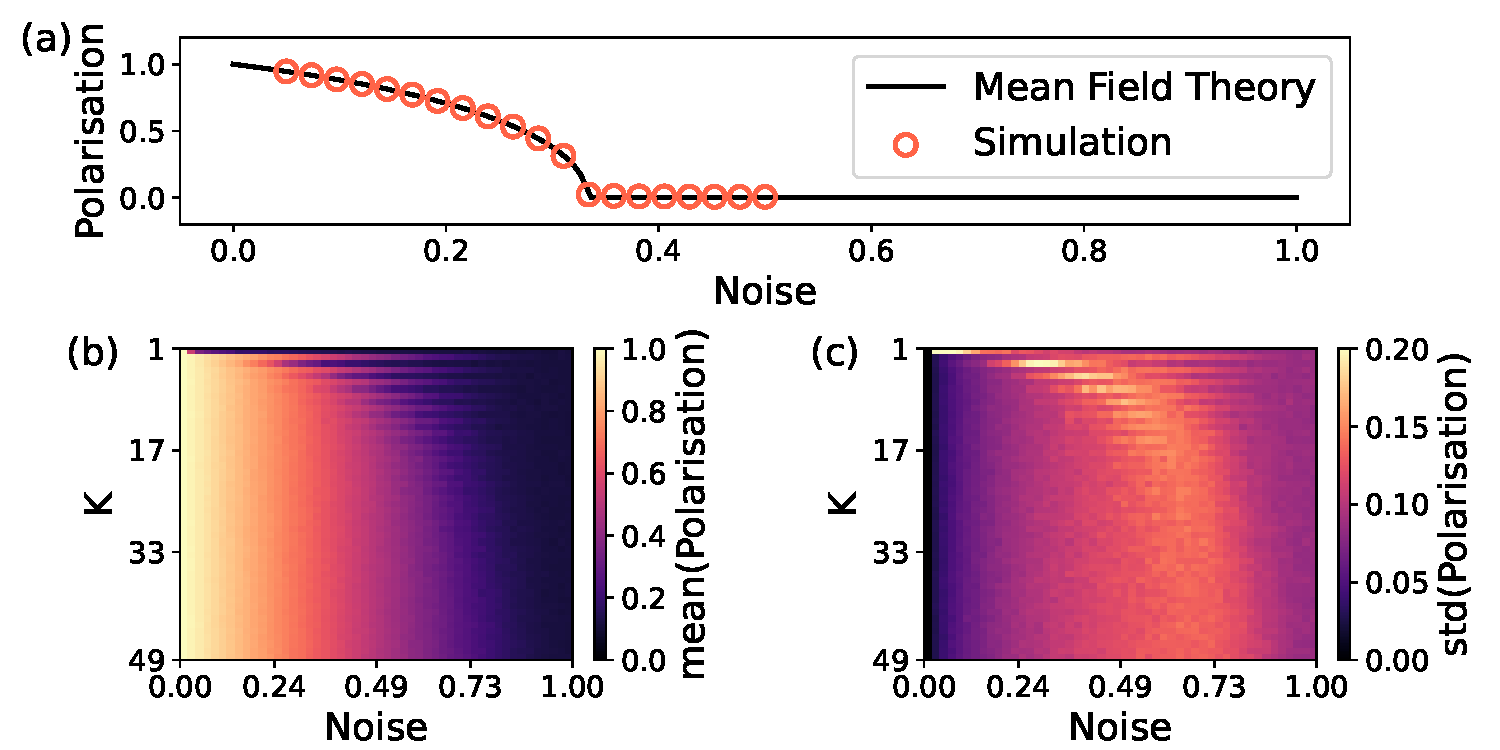
\includegraphics[width=\linewidth]{majority-voter}
  \caption{The behaviour of the voter model with intrinsic noise. (a) The relationship between the polarisation and the noise from the voter model ($K=3$). The scatters are the simulation result of a system ($N=50000$), and the solid line is the prediction of the mean--field theory \cite{pimentel2008PRE}. (b) The polarisation as a function of the connection number ($K$) and the noise. (c) The susceptibility as a function of the connection number ($K$) and the noise.}
  \label{fig:voter}
\end{SCfigure}

\subsection{The Vectorial Network Model}

For agents in the vectorial network model (VNM), their states were represented by a unit vector $\in R^d$, and the agents interact with each other through a random graph with fixed $K$ neighbours number, determined by its underlying graph.

This model is characterised by two parameters, the neighbour number $K$ and a noise term $\eta$, which randomly rotates the states of different agents. Increasing the parameter $K$ will increase the connection between different agents, hence guide the system to a more polarised macroscopic state. On the other hand, increasing the noise $\eta$ will reduce the order of the system, leading to random behaviour. This trend can be 


Let's call the VNM with the constrained graph cgVNM. The cgVNM is interesting because it is similar to the Vicsek model, where the interaction between agents were determined by their locations rather than a graph.


\section{Ordering in Real Space: Vicsek model and its derivatives}

The Vicsek model and its derivatives are famous model to describe the collective behaviour of animals, as review in section \ref{ch2-review-model}. These models are simple and they can relate to each other with a hierarchy. Here I will discuss three representative models, whose relationship can be summarised in Fig.\ \ref{fig:model-relation}. It is satisfying to discover that the ``most elementary'' model, the voter model, have a close relationship with the celebrated Ising model.


\subsection{The Vicsek Model}

The density in the Vicsek model is similar to the neighbour number in the VNM. And the phase diagram of the Vicsek model is very similar to that of the VNM.


\subsection{The modified Vicsek Model}

\subsection{The Inertial Spin Model}

\section{Realistic Ordering}

Even though the modified Vicsek model captured the relationship between the length scales and the polarisation of the zebrafish, a great amount of detail is lost. For instance, the spatial distribution in the Vicsek model is totally different from that of the real fish, for the lack of short--ranged repulsive interaction as well as the long ranged attraction. In addition, the biological details of the fish, such as the limited field--of--view, were not considered. This is not a bug, it is a feature. The simplicity of Vicsek model is indeed the reason for its popularity amongst the physics community. However, I still want to explore a bit further into the biological details, by constructing more realistic model to match the experiment. There is a trap of building a complicated model. Adding more parameters will make the model more realistic, but also increase our chance of \emph{overfitting}, where the model captured the irrelevant details (even measurement noises) rather than the general behaviour. Nevertheless, let us bravely march into the realm of the biology, where details of the model matter.

\subsection{The Couzin Model}

The well accepted realistic model for the behaviour of fish is proposed by Iain Couzin in 2002. It is hence called Couzin model. I implemented this model so that it can be used as a starting model, which is to be further modified to fit the experimental data of zebrafish.

\subsection{The Boundary}

The 3D geometry of the tank confining the zebrafish was determined in section \ref{section:system_3d}. Generally speaking, the shape of the tank can be expressed as,

$$
z = c r^2,
$$

\noindent where $c=0.734$ when both $r$ and $z$ were expressed in the unit of meters. The volume of the tank can be calculated as

$$
V = \int_{0}^{h}{\pi \frac{z}{c}} dz = \frac{\pi h^2}{2 c},
$$

\noindent where $h$ is the height of the tank, the vertical distance between the water surface and the base of the tank. The joint probability density function (PDF) of random points, being uniformly distributed inside the tank, is written as,

$$
f(x, y, z) = V^{-1} = \frac{2c}{\pi h^2}.
$$

\noindent From the expression we can calculate the marginal distribution of $x$ coordinates,

$$
\begin{aligned}
f_X(x) &= \int_{-\sqrt{h/c - x^2}}^{\sqrt{h/c - x^2}} dy
\int_{c(x^2 + y^2)}^{h} dz \; f(x, y, z) \\[1em]
&= \frac{8 c \sqrt{h/c-x^2} \left(h - c x^2 \right)}{3 \pi h^2}.
\end{aligned}
$$

\noindent The joint PDF of the uniform distribution can be expressed in the spherical coordinates as,

$$
f(\theta, r, z) = \frac{2c}{\pi h^2} r,
$$

\noindent where $\theta$ is the azimuth angle, $r = \sqrt{x^2 + y^2}$ is the radius in $XY$ plane. The marginal distribution of $r$ is written as,

$$
\begin{aligned}
f_R(r) &= \int_0^{2\pi}{d \theta} \int_{cr^2}^{h}{dz} \; f(\theta, r, z)
&= \frac{4c}{h} r - \frac{4 c^2}{h^2} r^3.
\end{aligned}
$$

\noindent Similarly, the marginal PDF of the $z$ component ($f_Z(z)$) is written as,

$$
\begin{aligned}
f_Z(z) &= \int_0^{2\pi}{d \theta} \int_0^{\sqrt{h/c}}{dr} \; f(\theta, r, z) 
&= \frac{2}{h^2} z.
\end{aligned}
$$

\begin{SCfigure}
  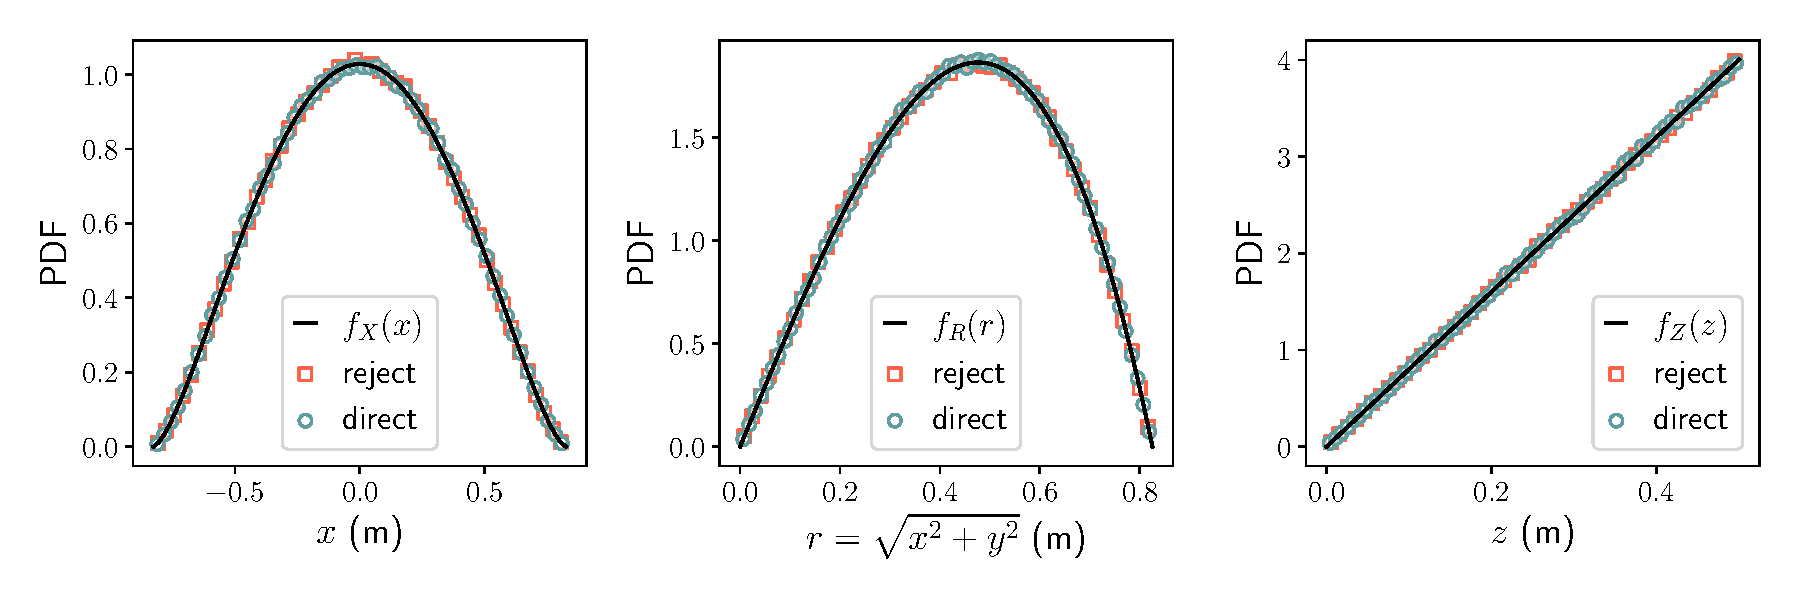
\includegraphics[width=\linewidth]{tank-marginal-dist}
  \caption{The marginal probability density distribution of points sampled uniformly inside the tank. Left: the distribution of x component of the points. Center: the distribution the radius in the XY plane. Right: the distribution of the z component of the points.}
  \label{fig:tank-dist}
\end{SCfigure}


\noindent The analytical result is checked against the numerical sampling of random points inside the tank, as shown in Fig.\ \ref{fig:tank-dist}. These PDFs can be used as comparison for the distribution of real fish data. The ratio of the PDFs, $\textrm{PDF}_\textrm{real} / \textrm{PDF}_\textrm{random}$, can be a measure of the effect of external field on the fish.

The interaction between the fish and the tank can take different forms. And there are two common options: alignment or reflection \cite{martinez2018}.

\subsection{The External Field}

The fish will be affected by the gravity. In fact, the fish always swims with their belly facing to the ground. But such behaviour 

\subsection{The Zebrafish Model}

\end{document}
